\section{Aktivenfahrt}
\sectionmark{Aktivenfahrt}

\begin{multicols}{2}

\textbf{„Bring Gott zum Lachen und mach Pläne!“}
sagt der Spruch – und das zu Recht. Obwohl unsere Aktivenfahrt abgesagt werden musste,
war sie trotzdem kein völliger Verlust. Persönlich hatte ich bis dahin noch
keinen deutschen Palast besucht, weshalb der Besuch des Schlosses Nymphenburg
doppelt großartig war. Es ist eines der bekanntesten Schlösser Bayerns und
liegt praktischerweise sogar näher an unserem Haus als das ursprüngliche
Fahrtziel.

Die Geschichte des Schlosses beginnt im Jahr 1664, als Kurfürst Ferdinand
Maria von Bayern den Bau eines Jagdschlosses für seine Frau, Herzogin Henriette
Adelaide von Savoyen, in Auftrag gab. Das ursprüngliche Gebäude wurde von den
Architekten Agostino Barelli und Enrico Zuccalli im Barockstil entworfen. Auf
jeden Fall kann man die italienische Atmosphäre in jedem Raum spüren!

Im Laufe des 18. Jahrhunderts wurde das Schloss unter den folgenden
Kurfürsten, insbesondere unter Maximilian II. Emanuel, erheblich erweitert und
verschönert. Im Jahr 1701 wurde der Schlossgarten im französischen Stil
angelegt, und auch verschiedene Pavillons und Gebäude wie das Pagodenhaus und
die Amalienburg kamen hinzu. Später, im 19. Jahrhundert, während der Herrschaft
König Ludwigs I. von Bayern, erlebte das Schloss eine weitere Umgestaltung.
Viele der Räume wurden im Stil des Rokokos und Klassizismus neu ausgestattet. Ludwig
I. nutzte Nymphenburg als Residenz und Kulturzentrum.

Heute beherbergt das Schloss mehrere Museen und Kunstsammlungen, darunter
das Marstallmuseum und das Porzellanmuseum, und ist ein beliebtes Ausflugsziel
– nicht nur für Touristen, sondern auch für zahlreiche Einheimische und
Zugvögel, die durch seine Seen, Kanäle und Gebäudeanlagen angezogen werden. Zwischen
den mit Holz überdachten Säulen und Statuen haben wir trotz des grauen
Novemberwetters schöne Bilder gemacht. Am Ende haben wir diesen wunderbaren Tag
natürlich mit einem Bier gekrönt.

Als ich meinen Kollegen im Labor von dieser Erfahrung erzählte, meinte
einer von ihnen, dass er so viel Prunk und Spektakel für oberflächlich und
nutzlos halte. Ich muss widersprechen. Eine solche Meinung ist heutzutage in
Europa weit verbreitet. Doch als jemand, der aus Südamerika stammt, weiß ich:
Die Überzeugung, dass das Schöne völlig entbehrlich ist, kann nur aus einem
Hintergrund entstehen, in dem Schönheit allgegenwärtig ist. Es ist zu einfach,
etwas zu unterschätzen, wenn es immer da ist!

	%
	\begin{flushright}
		\hfill\emph{Nicolas Delgado ?}
	\end{flushright}
	%	
\end{multicols}
%

%
\newpage
\begin{center}
		\begin{figurehere}
		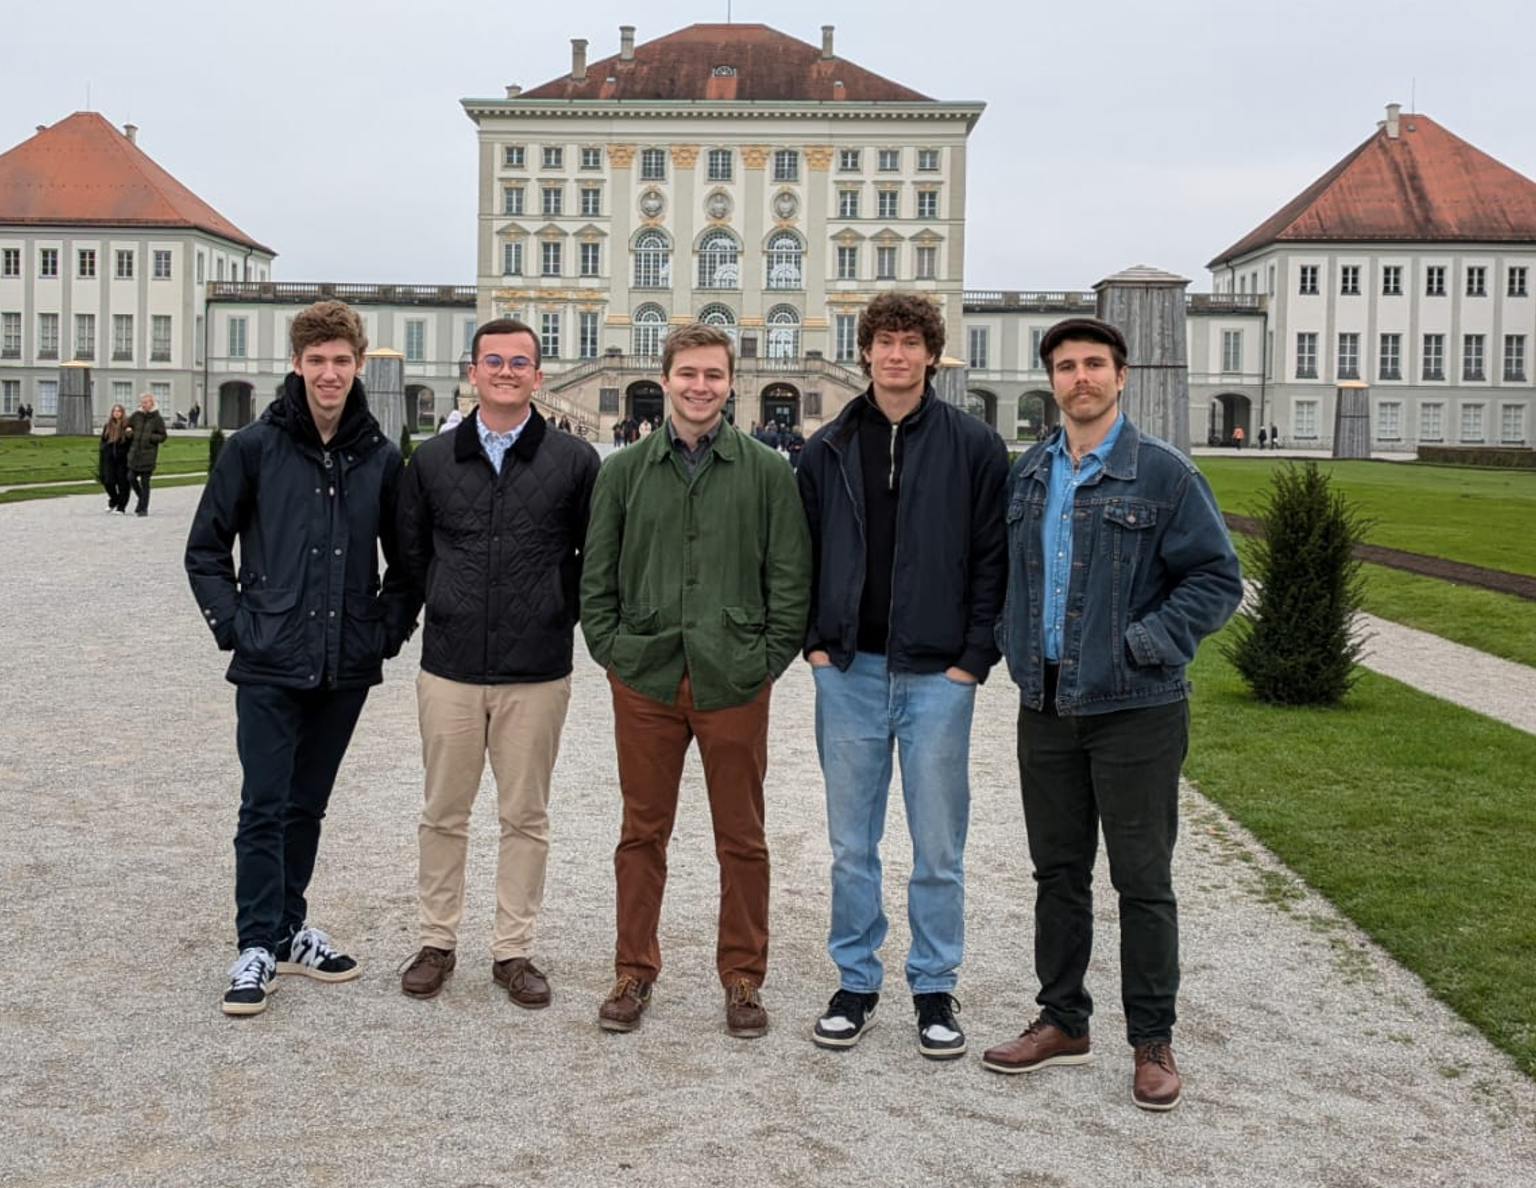
\includegraphics[width=.7\linewidth]{./Bilder/Neue Bilder/Aktivenfahrt/Aktivenfahrt}
		\end{figurehere}
\end{center}
	
